\documentclass[10pt, a4paper]{ieeeconf}

\overrideIEEEmargins

\usepackage[utf8]{inputenc}
\usepackage{tempora}
\usepackage{graphicx}
\usepackage{hyperref}
\usepackage{authblk}
\usepackage[english, russian]{babel}
\renewcommand*{\Affilfont}{\itshape}
\hypersetup{unicode=true}

\title{\LARGE \bf
Извлечение логической структуры из сканированных документов
}

\author{А.О. Богатенкова}
\affil{Институт системного программирования им. В.П. Иванникова \\
Российской академии наук, \\
Москва, Россия \\
bogatenkova.anastasiya@mail.ru}

\begin{document}

\maketitle
\thispagestyle{empty}
\pagestyle{empty}

%%%%%%%%%%%%%%%%%%%%%%%%%%%%%%%%%%%%%%%%%%%%%%%%%%%%%%%%%%%%%%%%%%%%%%%%%%%%%%%%

\begin{abstract}

Большое количество текстовой информации представлено в виде pdf-документов, у которых может отсутствовать текстовый слой. Зачастую требуется осуществлять быстрый поиск по их содержимому. Знание структуры документов может способствовать более эффективному их анализу.
В статье рассмотрены существующие решения задачи извлечения структуры документа в виде иерархии заголовков, а также предложен другой метод решения данной задачи, позволяющий отличать заголовки и элементы списков от остальных строк документа. Кроме того, размечен корпус документов, проведена экспериментальная проверка реализованного метода на данном корпусе и описаны возможности для дальнейшей работы и исследований.

\end{abstract}

\begin{keywords}

машинное обучение; структура документа; обработка естественного языка

\end{keywords}

%%%%%%%%%%%%%%%%%%%%%%%%%%%%%%%%%%%%%%%%%%%%%%%%%%%%%%%%%%%%%%%%%%%%%%%%%%%%%%%%

\section{ВВЕДЕНИЕ}

Как правило, документы имеют логическую структуру и содержат название, разбиение на главы, подглавы и т. д., нумерованные и маркированные списки. Выделение такой структуры документа может помочь при решении задач автоматизированного анализа документов, а также при поиске по документам.

Применяется множество разнообразных подходов \cite{link5,link6,link7}, которые позволяют выделять в тексте заголовки и распознавать логическую структуру документов. Однако данные подходы подразумевают работу с ограниченным количеством уровней вложенности и не принимают во внимание элементы списков. 

Ограничим класс рассматриваемых документов сканированными документами без текстового слоя. Будем считать, что в документах не содержатся изображения и таблицы. В данной статье описан метод извлечения структуры документа в виде заголовков, элементов списков и текстовых строк. Каждая строка документа относится к одному из этих трех типов на основе определённых признаков. Для выделения таких признаков может быть необходима метаинформация, такая как размер и тип шрифта, отступы, междустрочные интервалы и т. д. Поэтому извлечение логической структуры логично делать на этапе анализа сканированных документов.

Статья состоит из следующих частей: глава 2 содержит обзор различных подходов, с помощью которых решается задача выделения структуры документа; в главе 3 описывается датасет, используемый при реализации и проверке метода; в главе 4 рассматривается реализованный метод; в главе 5 показаны результаты экспериментальной проверки метода, а в главе 6 представлены краткие выводы и предлагаются возможности для дальнейшей работы и исследований.

\section{ОБЗОР АНАЛОГИЧНЫХ РАБОТ}

По извлечению структуры из документов существуют несколько подходов:
\begin{itemize}
\item на основе оглавления;
\item на основе правил;
\item на основе машинного обучения.
\end{itemize}

\subsection{Извлечение структуры из документов на основе оглавления и правил}

По анализу документов проводится очень много соревнований ICDAR, например \cite{link1,link2,link3}. В одном из таких соревнований \cite{link1} производилось извлечение структуры из книг, содержимое которых было получено с помощью оптического распознавания символов. Структура книг в виде разбиения на страницы, параграфы, главы извлекалась с использованием оглавления, которое присутствовало в большинстве книг. 

В 2019 году проводились соревнования FinTOC \cite{link4}, где из финансовых документов извлекалась структура в виде иерархии уровней заголовков документов. Максимальная глубина уровней равна пяти. Одна из команд-участниц \cite{link5} извлекала необходимую структуру используя оглавление документов, а также систему правил, которые применялись для определения иерархии заголовков.
Сначала идентифицировались страницы, содержащие текст оглавления, затем в документе находились страницы, соответствующие заголовкам, указанным в оглавлении. 
Последним шагом являлось выделение иерархии найденных заголовков, основанное на применении правил: анализировались такие признаки, как междустрочный интервал, отступ, шрифт, символы нумерации.
Использованный подход позволил получить достаточно высокую точность, но низкую полноту, так как некоторые оглавления документов были неполными.

Извлечение структуры документов на основе оглавления имеет ряд недостатков. Во-первых, невозможно обрабатывать документы, в которых нет оглавления. Во-вторых, при использовании этого метода в структуру документа не будут включаться заголовки, которые не вошли в оглавление, например заголовки более низкого уровня. В-третьих, данный метод не позволяет извлекать элементы маркированных и нумерованных списков, которые не включаются в оглавление документа.

\subsection{Извлечение структуры из документов на основе машинного обучения}

В соревнованиях \cite{link4} кроме извлечения иерархической структуры документов решалась задача определения, является ли конкретный блок документа заголовком. Командам был дан набор pdf-документов, xml-файлов с выделенными блоками документов, а так же набор признаков для каждого блока: является ли шрифт блока жирным, курсивом, состоит ли текст из заглавных букв, начинается с заглавной буквы или с нумерации. Кроме данных признаков, каждая из команд использовала различные дополнительные морфологические, семантические, лингвистические признаки. На основе этих признаков обучались различные классификаторы: SVM, MNB, Extra Tree, Decision Tree, Gradient Boosting. Для оценки результатов использовалась F1-мера, максимальный score в соревновании -- 0,982.

Победители соревнования \cite{link6} создали новый датасет для обучения с помощью аугментации данных, перевели новые сгенерированные текстовые блоки в векторное представление, а затем использовали рекуррентные нейронные сети LSTM и BiLSTM для решения задачи классификации. Процесс аугментации показан на рис. 1.

\begin{figure}[ht]
\center{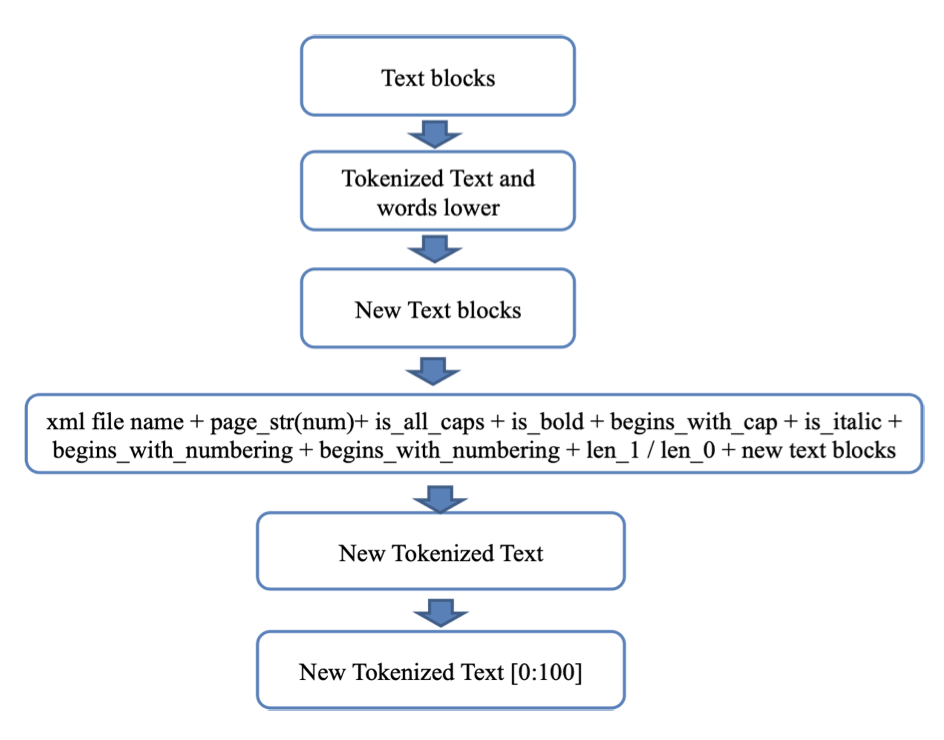
\includegraphics[width=0.5\textwidth]{pics/augmentation.png} }
\caption{Аугментация данных для LSTM и BiLSTM}
\end{figure}

В статье \cite{link7} 2017 года структура документа извлекалась с использованием методов машинного обучения, включая глубокое обучение. Цель данной работы -- автоматически идентифицировать и классифицировать различные секции документов и понять их смысл в рамках документа (назначить семантическую метку).

\begin{figure}[ht]
\center{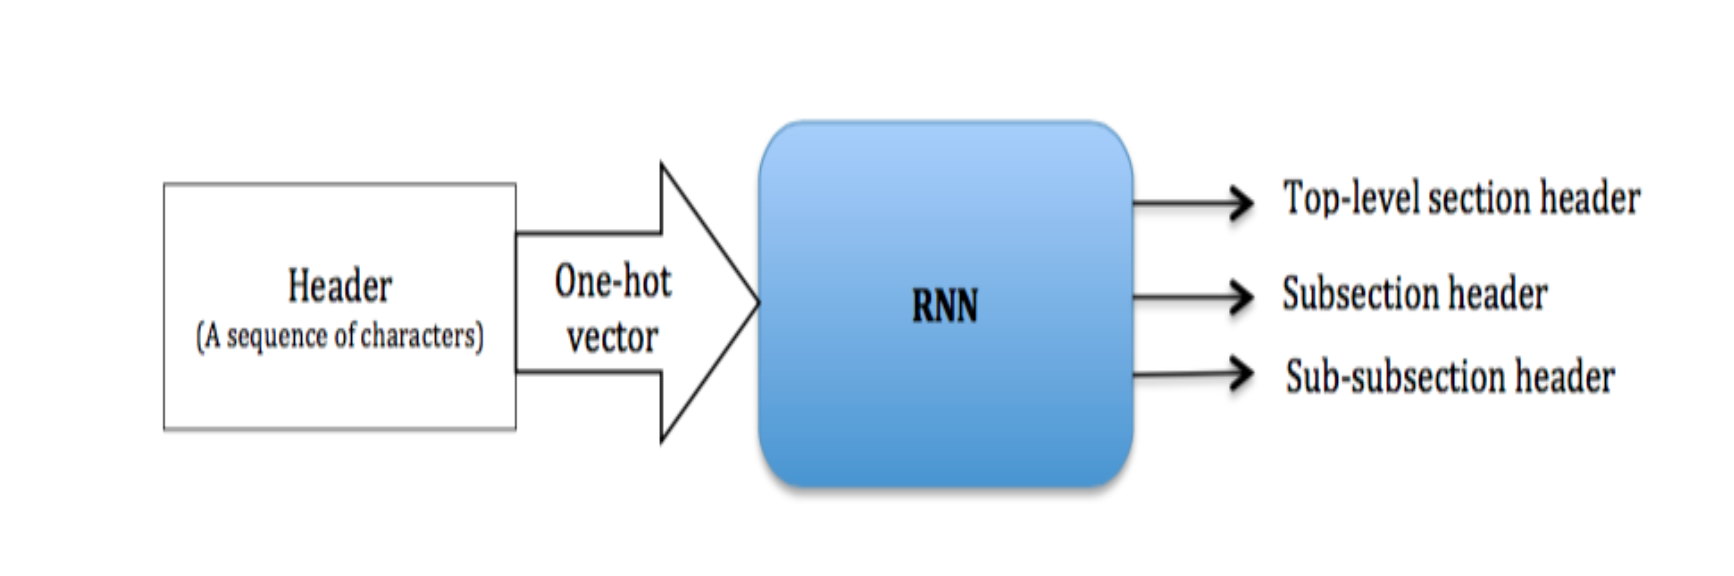
\includegraphics[width=0.5\textwidth]{pics/classifier.png} }
\caption{Вход и выход классификатора заголовков}
\end{figure}

Классификатор (рис. 2), который был использован при решении задачи, состоит из нескольких частей. Сначала строки документа подаются на вход классификатору (классификатор строк), который определяет, является ли строка заголовоком, затем строки-заголовки классифицируются точнее другими классификаторами (классификаторы секций). В этом решении структура документа имела вложенность 3, то есть предполагалось выделение секций, подсекций, подподсекций.
Кроме того, в данной работе был размечен датасет, на котором происходило обучение модели. Метрика качества - F1-мера, при идентификации заголовков итоговый score -- 0,96; при классификации секций средний F1-score -- 0,81.

\section{ДАТАСЕТ}

Датасет представляет собой набор документов в виде изображений в формате .jpeg, скачанный из интернета. Документы являются сканированными копиями текстов договоров различных предприятий (СТО, РД ЭО и др.). Каждое изображение будем считать отдельным документом.

Данный корпус имеет ряд специфических особенностей. Документы не содержат таблиц и рисунков, текст расположен строго по-горизонтали, не выделен цветом, шрифт не меняется (меняется только его начертание или размер). Большая часть всех текстов написана на русском языке, редко встречаются латинские буквы. Так как содержимое документов представляет собой в основном договоры предприятий, в текстах встречается большое количество элементов списков (нумерованных и маркированных), зачастую списки имеют очень глубокий уровень вложенности (четвертый, пятый). Заголовков относительно немного, они могут быть пронумерованы и также иметь глубокий уровень вложенности, поэтому их можно спутать с элементами списков.

Документы были размечены с использованием системы для разметки, разработанной в ИСП РАН \cite{link8}. Текст документов распознавался с помощью программы Tesseract \cite{link10}.  Результатом разметки стал набор .json файлов, каждый из которых содержит название документа и список текстовых строк. Для каждой строки указаны координаты заключающей её рамки (bounding box) и правильная метка.

Для проверки правильности разметки была посчитана специальная статистика \href{https://en.wikipedia.org/wiki/Cohen%27s_kappa}{Cohen's kappa}. После разметки десяти документов двумя аннотаторами значение статистики $\kappa$ оказалось равным 0.975 (чем ближе значение $\kappa$ к единице, тем больший уровень согласия достигнут между аннотаторами), после чего было решено размечать остальной корпус документов. В результате было размечено 600 документов и отдельные .json файлы были объединены в один.

\section{ОПИСАНИЕ РЕШЕНИЯ}

\subsection{Выделение признаков}

Среди признаков, характеризующих строки документа, можно выделить следующие группы:

\begin{itemize}

  \item Признаки, основанные на регулярных выражениях.

  Данная группа признаков основывается на анализе начала и конца каждой строки. Такие признаки очень важны для выявления элементов списков различных типов, а также могут сигнализировать о конце заголовка или начале списка.

  Регулярные выражения позволяют выделить следующие признаки:
  \begin{itemize}

    \item[--] начинается ли строка с цифры или буквы со скобкой или точкой (также анализируются иерархические выражения вида 1.1.1);
    \item[--] начинается ли строка с тире (и других символов, характерных для маркированного списка);
    \item[--] состоит ли строка целиком из заглавных букв (характерно для некоторых заголовков);
    \item[--] начинается ли строка с заглавной (строчной) буквы;
    \item[--] начинается ли строка с конкретных слов типа «Раздел», «Секция», «Глава» и т. д.;
    \item[--] оканчивается ли строка символами вида «. , ; :»;
    \item[--] оканчивается ли строка строчной буквой.

  \end{itemize}

  \item Текстовые признаки.

  Данная группа признаков связана с подсчетом некоторых строковых характеристик, а именно:

  \begin{itemize}

    \item[--] количество букв в первом и втором словах строки;
    \item[--] количество слов в строке (строка разбивается на слова по пробелам);
    \item[--] количество символов в строке (длина строки).

  \end{itemize}

  \item Визуальные признаки.

  Данная группа признаков связана с графическим представлением текста в документе. То есть при анализе строки рассматривается не ее текст, а следующие признаки:

  \begin{itemize}

    \item[--] отступ от левого края страницы;
    \item[--] высота текста строки (точнее высота ограничивающей ее рамки);
    \item[--] отступ от верхнего края страницы;
    \item[--] жирность шрифта различных уровней.

  \end{itemize}

\end{itemize}

Кроме того, к признакам, перечисленным выше, для каждой строки были добавлены аналогичные признаки четырех предыдущих и следующих строк. Это нужно для анализа продолжения блока строк конкретного типа.

Для строк, которые начинаются с нумерации, определялось, есть ли в документе строка, предшествующая данной с нумерацией, меньшей данной на единицу.

И, наконец, для каждого документа вычислялся средний отступ от левого края страницы, средняя высота шрифта, средняя длина строки, среднее число слов в строках, среднее значение дли жирности шрифта, среднее число букв в первом слове каждой строки. Данные значения добавлялись к признакам каждой строки документа.

\subsection{Подбор классификатора}

При решении задачи было опробовано множество классификаторов, для лучших из них проведен анализ результатов. В анализе участвовало 4 классификатора:

\begin{itemize}

  \item алгоритм k ближайших соседей (\href{https://scikit-learn.org/stable/modules/generated/sklearn.neighbors.KNeighborsClassifier.html}{KNeighborsClassifier});
  \item логистическая регрессия (\href{https://scikit-learn.org/stable/modules/generated/sklearn.linear_model.LogisticRegression.html}{LogisticRegression});
  \item градиентный бустинг (\href{https://scikit-learn.org/stable/modules/generated/sklearn.ensemble.GradientBoostingClassifier.html}{GradientBoostingClassifier});
  \item экстра-градиентный бустинг (\href{https://xgboost.readthedocs.io/en/latest/}{XGBClassifier}).

\end{itemize}

Множество документов тремя способами было разбито на тренировочное и тестовое множества (разбиение по документам), на каждом разбиении было проведено обучение классификаторов и вычисление F1-score. Усредненные значения F1-score для каждого классификатора указаны в таблице 1.
\begin{table}[h]
\begin{center}
\begin{tabular}{ |p{3cm}||p{3cm}| }
 \hline
 \bf Классификатор & \bf F1-score \\
 \hline
 \hline
 Nearest Neighbors & 0.89\\
 \hline
 Logistic Regression& 0.9\\
 \hline
 Gradient Boosting & 0.92\\
 \hline
 \bf XGBoost & \bf 0.95\\
 \hline
\end{tabular}
\end{center}
\caption{Сравнение классификаторов}
\end{table}

В целом, все рассмотренные классификаторы показали хороший результат, наилучший результат показал XGBClassifier, поэтому было решено выбрать его.

\subsection{Анализ значимости признаков}

В таблице 2 представлены первые 10 признаков с наивысшей значимостью (information gain). Это признаки, которые имеют наибольший вес при вычислении предсказания классификатора.

\begin{table}[h]
\begin{center}
\begin{tabular}{ |p{4cm}||p{2cm}| }
 \hline
 \bf Признак & \bf Information gain \\
 \hline
 \hline
 Число символов первого слова в строке & 22089\\
 \hline
 Индикатор, является ли строка продолжением списка & 2400\\
 \hline
 Жирность шрифта & 2368\\
 \hline
 Число слов в строке & 2263\\
 \hline
 Отступ от левого края страницы & 1157\\
 \hline
 Признак начала строки с выражения вида 1.1.1 (произвольный уровень вложенности, вместо цифр могут быть буквы) & 1519\\
 \hline
 Жирность шрифта (менее жирный шрифт) & 811\\
 \hline
 Индикатор, заканчивается ли предыдущая строка буквой & 611\\
 \hline
 Число букв в начале строки & 361\\
 \hline
 Тире в начале строки & 359\\
 \hline
\end{tabular}
\end{center}
\caption{Значимость признаков}
\end{table}

С использованием данных о важности признаков, в признаковое пространство были добавлены новые признаки. Например, вместо одного признака, отвечающего за жирность шрифта, была добавлена целая группа признаков, отвечающая за различные уровни жирности шрифта. Для самых важных признаков к вектору признаков каждой строки документа были добавлены усреднённые значения данных признаков по документу. В таблице 2 представлен итоговый список признаков и значения их важности.

\section{РЕЗУЛЬТАТЫ}

После настройки параметров XGBClassifier ($learning\_rate$, $n\_estimators$, $max\_depth$, $min\_child\_weight$,
$gamma$, $subsample$, $colsample\_bytree$, $alpha$) итоговый F1-score, полученный в результате кросс-валидации оказался равным 0.98995. 

На рис. 3 показана \href{https://en.wikipedia.org/wiki/Confusion_matrix}{матрица ошибок} для полученного классификатора. По вертикальной оси расположены правильные классы, по горизонтальной - классы, которые предсказал классификатор. В клетках на пересечении расположены значения количества строк, у которых совпали данные классы.

\begin{figure}[ht]
  \center{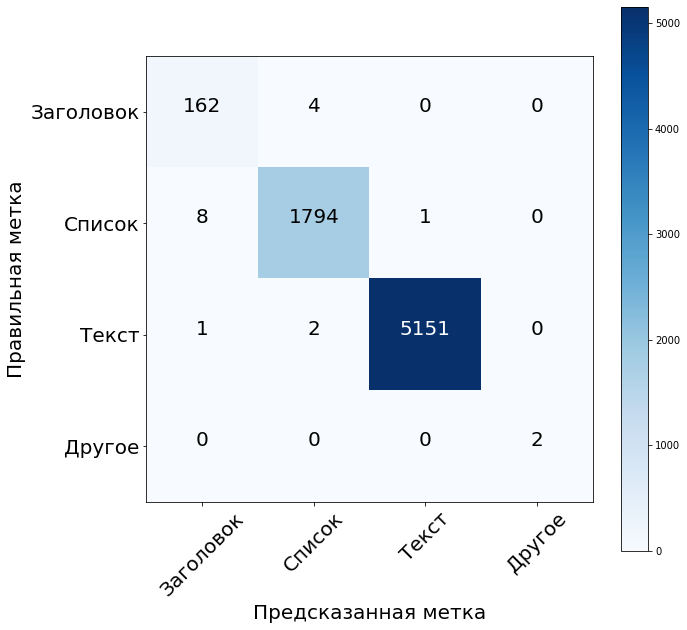
\includegraphics[width=0.45\textwidth]{pics/conf_matrix_rus.png}}
  \caption{Матрица ошибок без нормализации}
\end{figure}

На рисунке видно, что 8 строк, относящихся к типу «Список», были проклассифицированы как «Заголовок», 4 строки, напротив, вместо метки «Заголовок» получили метку «Список». Аналогичную статистику можно посмотреть и для других пар классов.

Таким образом, больше всего классификатор путает классы «Заголовок» и «Список». Это можно объяснить тем, что некоторые признаки данных классов очень похожи, например, многие заголовки начинаются с нумерации, а элементы списков имеют большой отступ от левого края страницы.

\section{ВЫВОДЫ}

В данной статье реализован метод выделения логической структуры документа, основанный на классификации строк документа, определяющий в документах заголовки и списки разных уровней вложенности.

Был размечен копус документов, используемый в качестве тренировочных данных, выявлены признаки, наиболее подходящие для классификации строк документа. Для классификации использован XGBClassifier, для которого были подобраны оптимальные параметры. Итоговый F1-score, полученный при настройке параметров, равен 0.98995. В силу особенностей датасета классификатор чаще всего путает заголовки и элементы списков.

Дальнейшие исследования могут быть направлены на выделение более подробной структуры. Помимо классификации каждой строки можно определять её уровень вложенности по отношению к документу.

\begin{thebibliography}{99}

\bibitem{link1} \href{https://hal.archives-ouvertes.fr/hal-01073396/document}{Doucet A. et al. ICDAR 2013 competition on book structure extraction //2013 12th International Conference on Document Analysis and Recognition. – IEEE, 2013. – С. 1438-1443.}
\bibitem{link2} \href{https://ieeexplore.ieee.org/abstract/document/8270162}{Gao L. et al. ICDAR2017 competition on page object detection //2017 14th IAPR International Conference on Document Analysis and Recognition (ICDAR). – IEEE, 2017. – Т. 1. – С. 1417-1422.}
\bibitem{link3} \href{https://usir.salford.ac.uk/id/eprint/44369/1/ICDAR2017%20Competition%20on%20Recognition%20of%20Documents%20with%20Complex%20Layouts.pdf}{Clausner C., Antonacopoulos A., Pletschacher S. Icdar2017 competition on recognition of documents with complex layouts-rdcl2017 //2017 14th IAPR International Conference on Document Analysis and Recognition (ICDAR). – IEEE, 2017. – Т. 1. – С. 1404-1410.}
\bibitem{link4} \href{https://www.aclweb.org/anthology/W19-6407.pdf}{Juge R., Bentabet I., Ferradans S. The fintoc-2019 shared task: Financial document structure extraction //Proceedings of the Second Financial Narrative Processing Workshop (FNP 2019). – 2019. – С. 51-57.}
\bibitem{link5} \href{https://www.aclweb.org/anthology/W19-6409.pdf}{Giguet E., Lejeune G. Daniel@ FinTOC-2019 Shared Task: TOC Extraction and Title Detection //Proceedings of the Second Financial Narrative Processing Workshop (FNP 2019). – 2019. – С. 63-68.}
\bibitem{link6} \href{http://www.ep.liu.se/ecp/165/001/ecp19165001.pdf}{Tian K., Peng Z. Finance document Extraction Using Data Augmentation and Attention //Proceedings of the Second Financial Narrative Processing Workshop (FNP 2019), September 30, Turku Finland. – Linköping University Electronic Press, 2019. – №. 165. – С. 1-4.}
\bibitem{link7} \href{https://dl.acm.org/doi/pdf/10.1145/3148055.3148080}{Rahman M. M., Finin T. Deep Understanding of a Document's Structure //Proceedings of the Fourth IEEE/ACM International Conference on Big Data Computing, Applications and Technologies. – 2017. – С. 63-73.}
\bibitem{link8} \href{https://github.com/dronperminov/ParagraphLabelerApp}{ParagraphLabelerApp}
\bibitem{link10} \href{https://research.google/pubs/pub33418.pdf}{Smith R. An overview of the Tesseract OCR engine //Ninth International Conference on Document Analysis and Recognition (ICDAR 2007). – IEEE, 2007. – Т. 2. – С. 629-633.}
\bibitem{link9} \href{https://www.analyticsvidhya.com/blog/2016/03/complete-guide-parameter-tuning-xgboost-with-codes-python/}{Complete Guide to Parameter Tuning in XGBoost with codes in Python}

\end{thebibliography}

\end{document}
